\documentclass[border=10pt]{standalone}
\usepackage{pgfplots}
\usetikzlibrary{arrows.meta, shapes, calc}

\begin{document}
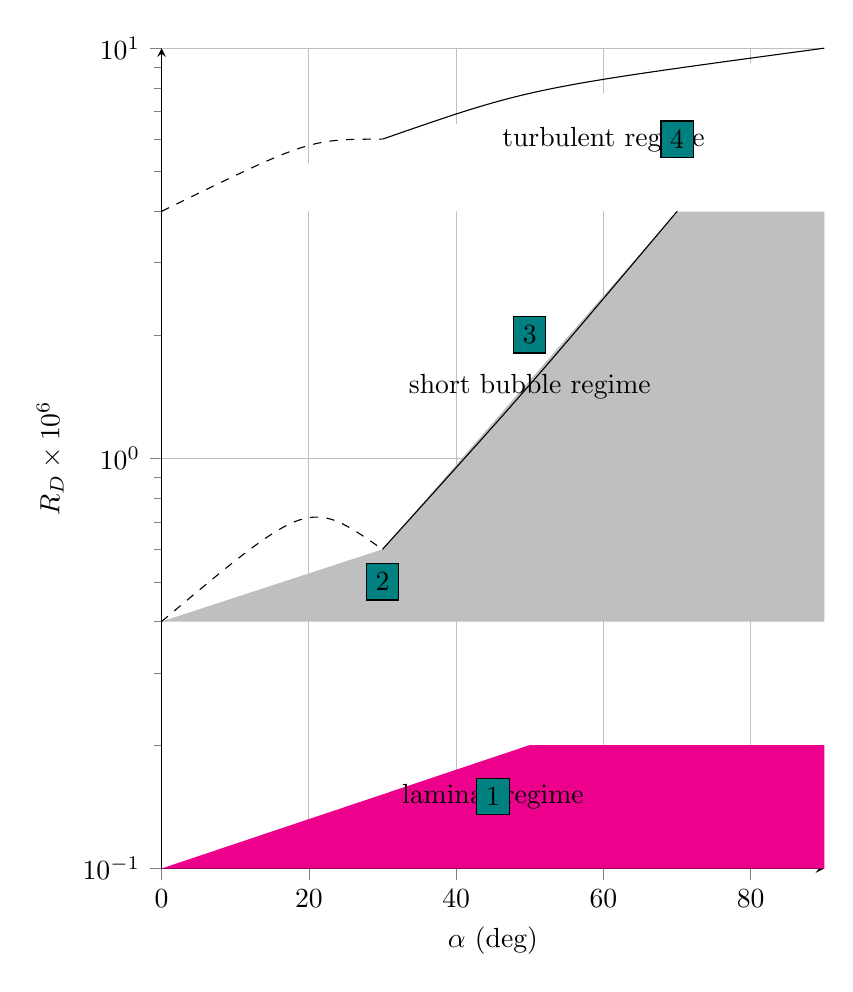
\begin{tikzpicture}
    \begin{axis}[
        width=10cm,
        height=12cm,
        xlabel={$\alpha$ (deg)},
        ylabel={$R_D \times 10^6$},
        xmin=0, xmax=90,
        ymin=0.1, ymax=10,
        ymode=log,
        grid=major,
        axis lines=left,
        tick align=outside,
        enlargelimits=false,
        clip=false,
        ]

        % Laminar regime
        \fill[magenta] (axis cs:0,0.1) -- (axis cs:50,0.2) -- (axis cs:90,0.2) -- (axis cs:90,0.1) -- cycle;
        \node at (axis cs:45,0.15) {laminar regime};
        
        % Short bubble regime
        \fill[gray!50] (axis cs:0,0.4) -- (axis cs:30,0.6) -- (axis cs:70,4) -- (axis cs:90,4) -- (axis cs:90,0.4) -- cycle;
        \node at (axis cs:50,1.5) {short bubble regime};
        
        % Turbulent regime
        \fill[white] (axis cs:0,4) -- (axis cs:30,6) -- (axis cs:90,10) -- (axis cs:90,4) -- cycle;
        \node at (axis cs:60,6) {turbulent regime};
        
        % Boundaries
        \draw[dashed] (axis cs:0,0.4) .. controls (axis cs:20,0.8) .. (axis cs:30,0.6);
        \draw (axis cs:30,0.6) .. controls (axis cs:50,1.5) .. (axis cs:70,4);
        \draw[dashed] (axis cs:0,4) .. controls (axis cs:20,6) .. (axis cs:30,6);
        \draw (axis cs:30,6) .. controls (axis cs:50,8) .. (axis cs:90,10);
        
        % Points
        \node[draw, fill=teal, minimum size=0.3cm] at (axis cs:45,0.15) {1};
        \node[draw, fill=teal, minimum size=0.3cm] at (axis cs:30,0.5) {2};
        \node[draw, fill=teal, minimum size=0.3cm] at (axis cs:50,2) {3};
        \node[draw, fill=teal, minimum size=0.3cm] at (axis cs:70,6) {4};
        
    \end{axis}
\end{tikzpicture}
\end{document}